\documentclass{article}
\usepackage{fullpage}
\usepackage[czech]{babel}
\usepackage{amsfonts}
\usepackage{graphicx}
\usepackage{caption}

\title{\vspace{-2cm}Francie, Apeninský poloostrov a Svatá říše římská\vspace{-1.7cm}}
\date{}

\begin{document}
\maketitle
\section*{Francie}
\begin{minipage}{0.6\textwidth}
    \subsection*{Karlovci (do 987)}
    \begin{itemize}
        \vspace{-0.5em}
        \setlength\itemsep{0.15em}
        \item[$-$] šlechta si vymohla \textit{léno} (dědictví) na Karlu II.
        \item[$-$] Normanské vévodství (911 -- 1259), pojmenované podle Vikingů (Normané), smlouva mezi \textbf{Karlem III. Prosťáčkem} a vikingským vojevůdcem \textbf{Rollem} toto vévodství ustanovila, po r. 1259 je součást Francie
    \end{itemize}

    \subsection*{Kapetovci (987 -- 1328)}
    \begin{itemize}
        \vspace{-0.5em}
        \setlength\itemsep{0.15em}
        \item[$-$] \textbf{Hugo Kapet} (987 -- 996)
            \begin{itemize}
                \vspace{-0.5em}
                \setlength\itemsep{0.15em}
                \item[$-$] vévoda Île-de-France (centrální část Francie, okolo Paříže)
                \item[$-$] později jmenován králem Francie (\textit{rex francorum})
            \end{itemize}
    \end{itemize}

    \subsection*{Francouzská společnost}
    \begin{itemize}
        \vspace{-0.5em}
        \setlength\itemsep{0.15em}
        \item[$-$] boj královská moc vs. šlechta, panovník vs. církev
        \item[$-$] feudální rozdrobenost
        \item[$-$] klášter Cluny (Clunijské hrabství)
        \item[$-$] \textit{boží příměří} -- zákon zakazující války ve svátky
        \item[$-$] města jsou nezávislá na církvi a šlechtě, jen na králi
    \end{itemize}
\end{minipage}
\hfill
\noindent\begin{minipage}{0.3\textwidth}
    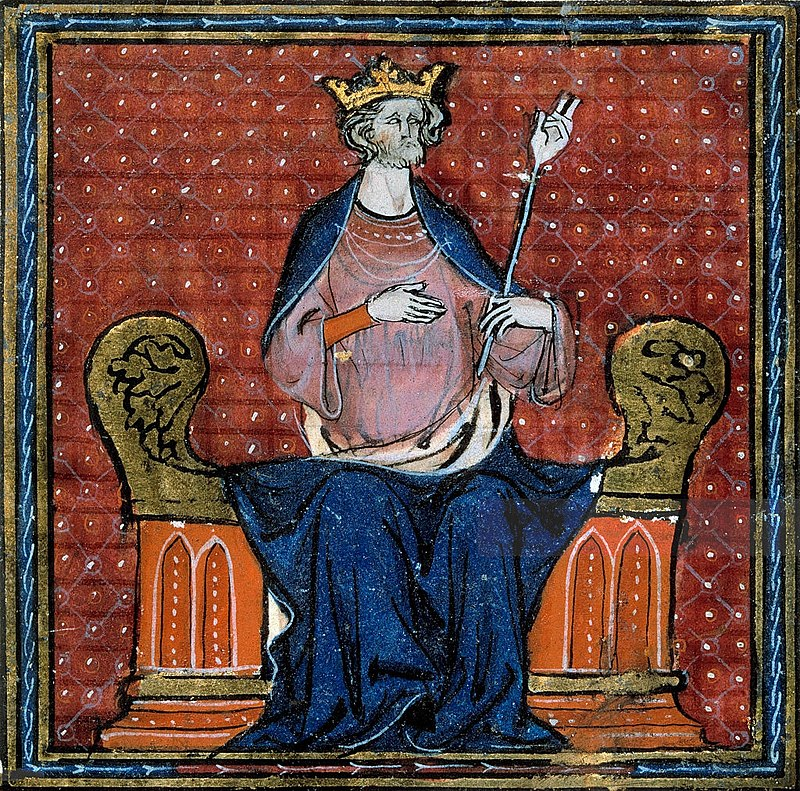
\includegraphics[width=\linewidth]{hugo_kapet.jpg}
    \captionof{figure}{Hugo Kapet}
    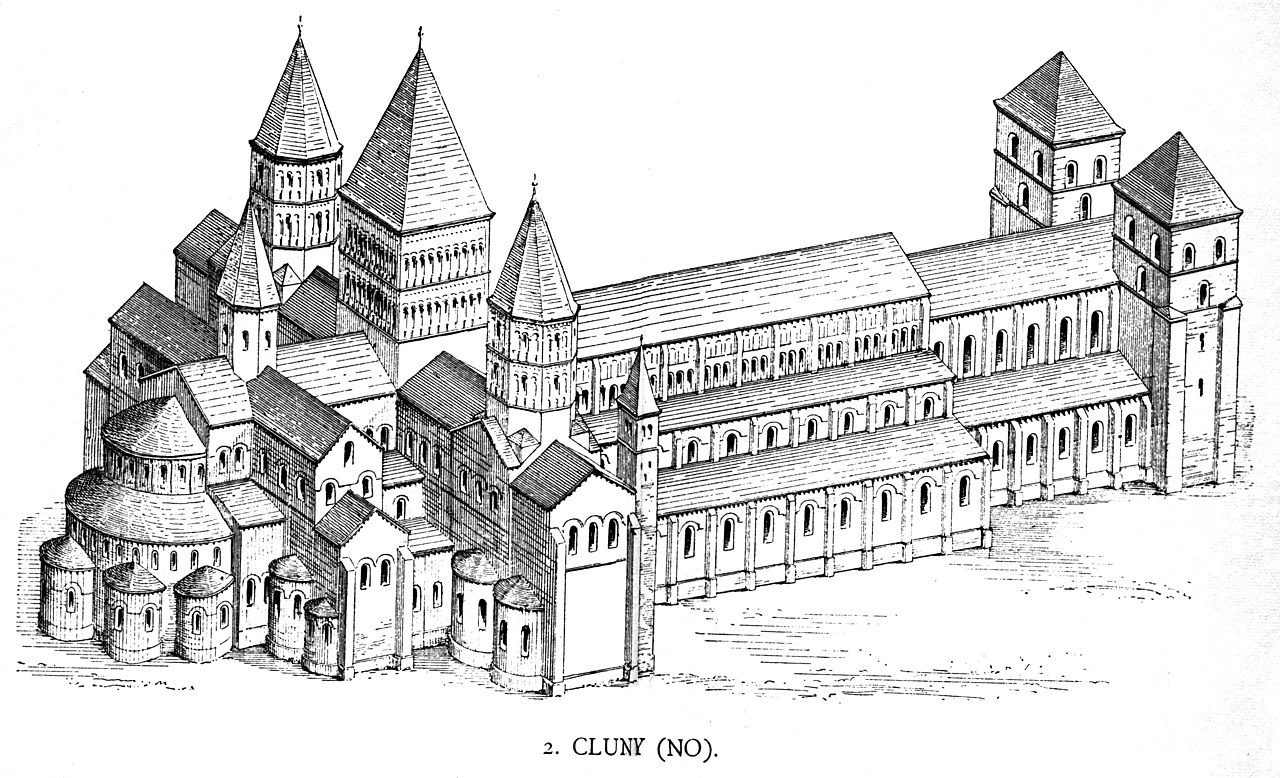
\includegraphics[width=\linewidth]{klaster_cluny.jpg}
    \captionof{figure}{klášter Cluny}
\end{minipage}

\section*{Apeninský poloostrov}
\begin{minipage}{0.6\textwidth}\raggedleft
    \begin{itemize}
        \vspace{-0.5em}
        \setlength\itemsep{0.15em}
        \item[$-$] útoky okolních národů (Arabové, Normani) $\rightarrow$ rozpadnutí na jednotlivé části, feudální rozdrobenost
        \item[$-$] Burgundské království, od 11. st. SŘŘ, ve 14. st. postoupeno Francii
        \item[$-$] Benátská republika -- u moci měšťané, v čele \textit{dóže}, námořní velmoc
        \item[$-$] Papežský stát (\textit{papa} = otec), první biskup sv. Petr, \textit{Konstantinova donace} = měl biskupům zaručovat nadvládu nad Římem, bohužel ne $\rightarrow$ \textit{Pipinova donace} = potvrzuje nároky papežů, Pipin na oplátku uznán za vládce Franské říše; papežové voleni šlechtou, papež Silvestr II.: \textit{renovation imperii} -- obnovení SŘŘ
    \end{itemize}
\end{minipage}
\hfill
\noindent\begin{minipage}{0.3\textwidth}
    \vspace{-3em}
    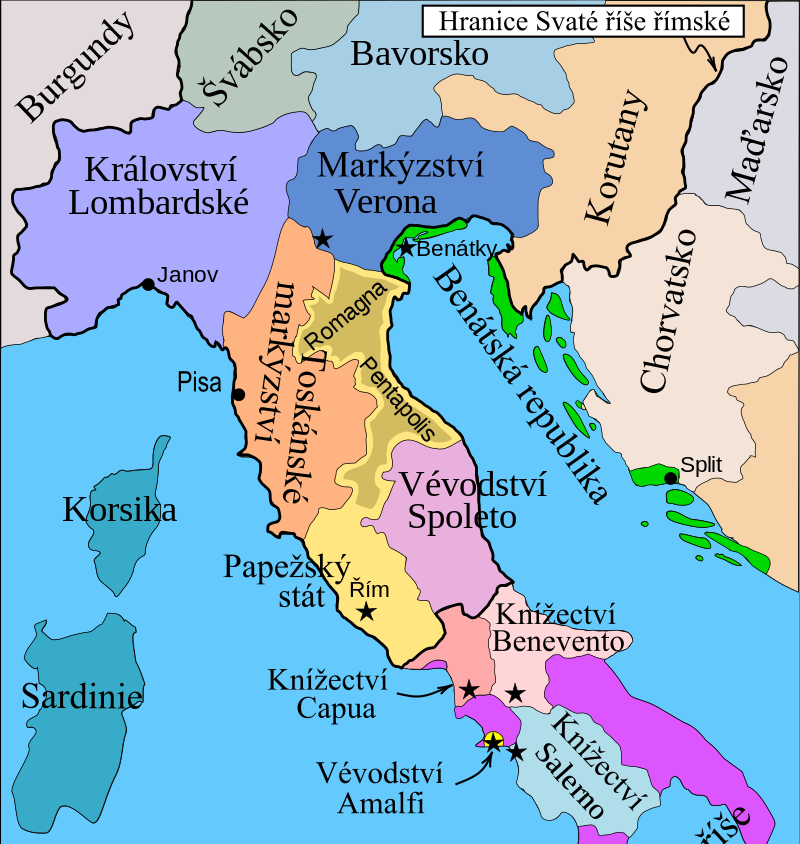
\includegraphics[width=\linewidth]{ap_pol.png}
    \captionof{figure}{Apeninský pol. kolem roku 1000}
\end{minipage}

\section*{Svatá říše římská = SŘŘ (do 1806)}
\begin{minipage}{0.6\textwidth}
    \vspace{-3em}
    \subsection*{Karlovci (do 918)}
    \begin{itemize}
        \vspace{-0.5em}
        \setlength\itemsep{0.15em}
        \item[$-$] \textbf{Ludvík II. Němec}
        \item[$-$] \textbf{Karel III. Tlustý} chce sjednotit Franskou říši (Bavorsko, Sasko, Frankové, Švábsko, \dots), neúspěch
    \end{itemize}
\end{minipage}
\hfill
\noindent\begin{minipage}{0.3\textwidth}
    \vspace{-3.5em}
    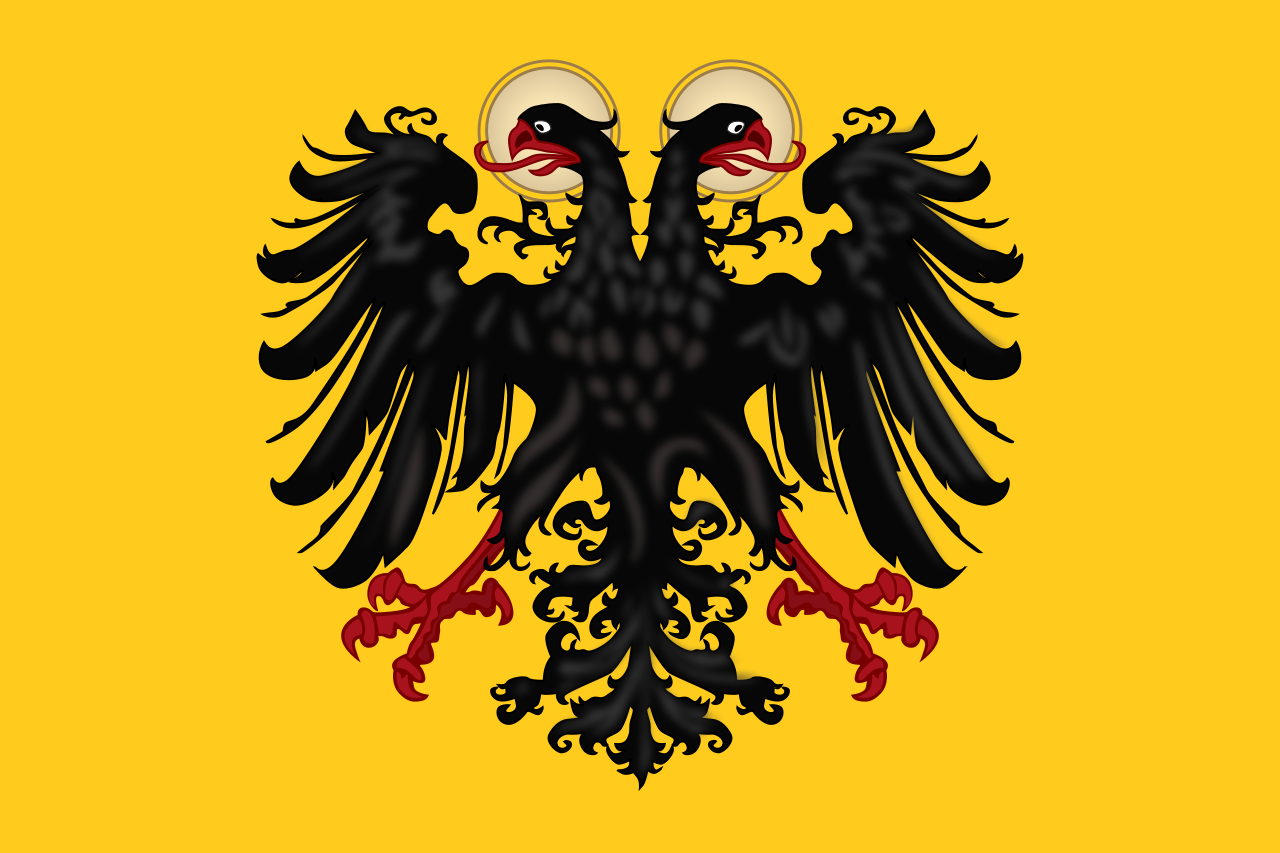
\includegraphics[width=\linewidth]{vlajka.png}
    \captionof{figure}{Vlajka SŘŘ}
\end{minipage}

\begin{minipage}{0.6\textwidth}
    \subsection*{Rod Otonů (919 -- 1023)}
    \begin{itemize}
        \vspace{-0.5em}
        \setlength\itemsep{0.15em}
        \item[$-$] \textbf{Jindřich I. Ptáčník} (919 -- 936)
            \begin{itemize}
                \vspace{-0.5em}
                \setlength\itemsep{0.15em}
                \item[$-$] zvolen
                \item[$-$] připojil Lotrinské království
                \item[$-$] Maďaři dělají problémy, útočí
            \end{itemize}
        \item[$-$] SŘŘ sestává z: německé státy, České království, Italské království, Papežský, stát, dočasná území (Švýcarsko, Lucembursko)
        \item[$-$] \textbf{Otto I.} (936 -- 973)
            \begin{itemize}
                \vspace{-0.5em}
                \setlength\itemsep{0.15em}
                \item[962] císařem, \textit{římská císařská jízda}
                \item[955] \textsc{bitva u Lešských polí}, porážka Maďarů
                \item[$-$] expanze: S Itálie, V -- Z Slované
            \end{itemize}
        \item[$-$] \textbf{Otto II.} (973 -- 983)
            \begin{itemize}
                \vspace{-0.5em}
                \setlength\itemsep{0.15em}
                \item[$-$] mírové vztahy s Byzancí
            \end{itemize}
        \item[$-$] \textbf{Otto III.} (983 -- 1002)
            \begin{itemize}
                \vspace{-0.5em}
                \setlength\itemsep{0.15em}
                \item[$-$] chce obnovit říši, \textit{renovation imperii}
                \item[$-$] papež \textbf{Silvestr II.} -- zavedení arabských číslic, založeno Uherské a Polské arcibiskupství
                \item[$-$] současník \textbf{sv. Vojtěch} -- šíří křesťanství, poslední Slavníkovec, druhý biskup pražský
                \item[$-$] po jejich smrti myšlenka o obnovení říše zaniká
                \item[$-$] začíná \textit{boj o investituru} mezi papežem a králem, kdo bude dominovat, naplno za Sálské dynastie
            \end{itemize}
    \end{itemize}
\end{minipage}
\hfill
\noindent\begin{minipage}{0.3\textwidth}
    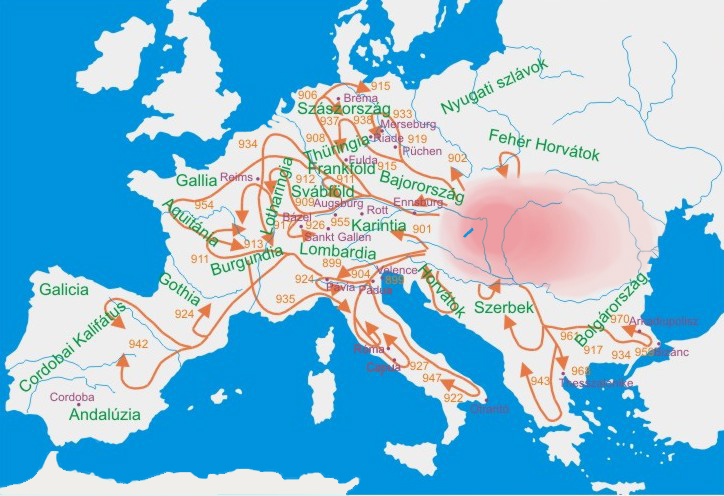
\includegraphics[width=\linewidth]{madari.jpg}
    \captionof{figure}{Nájezdy Maďarů v 10. st.}
    \vspace{1em}
    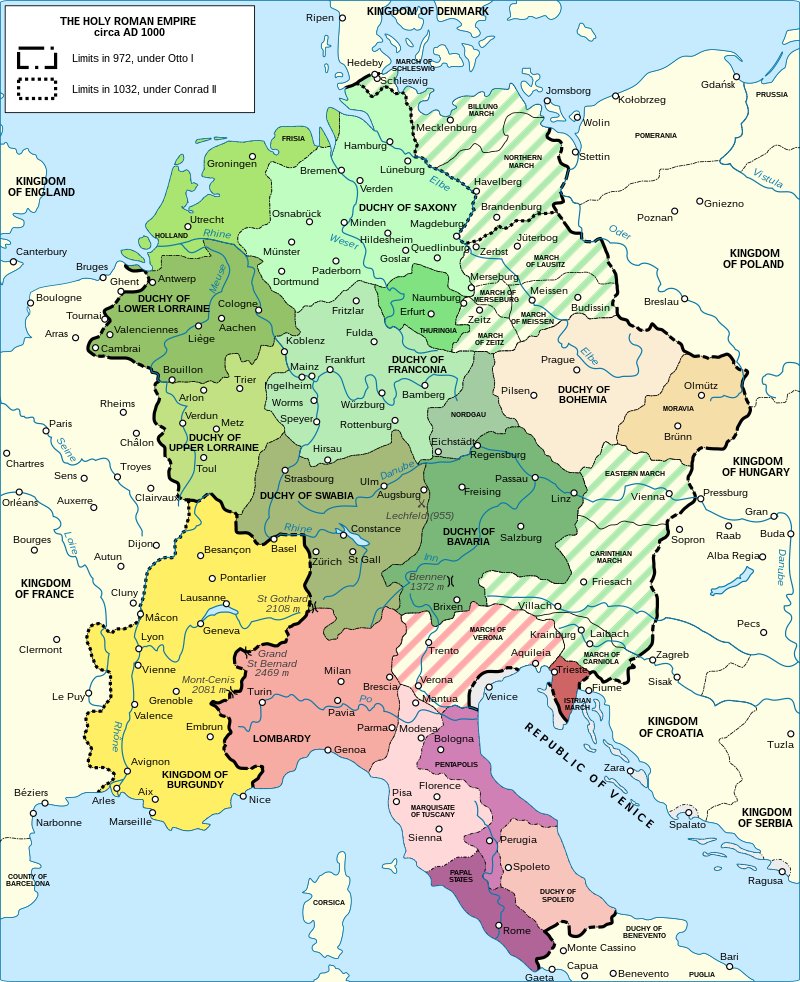
\includegraphics[width=\linewidth]{srr_mapa_10.png}
    \captionof{figure}{Území SŘŘ v 11. st.}
\end{minipage}

\subsection*{Sálská dynastie (1024 -- 1125)}
\begin{minipage}{0.6\textwidth}
    \begin{itemize}
        \vspace{-0.5em}
        \setlength\itemsep{0.15em}
        \item[$-$] souboj mezi papežem a králem
        \item[$-$] papež \textbf{Řehoř VII.}
            \begin{itemize}
                \vspace{-0.5em}
                \setlength\itemsep{0.15em}
                \item[(1073)] zvolen papežem
                \item[(1075)] sepsal tzv. \textit{Dictatus papae} (papežská bula) -- chce mít možnost dosazovat i odvolávat biskupy a panovníky
            \end{itemize}
        \item[$-$] král \textbf{Jindřich IV.}
            \begin{itemize}
                \vspace{-0.5em}
                \setlength\itemsep{0.15em}
                \item[$-$] s papežskou bulou nesouhlasí, svolá seszení církevních hodnostářů = \textit{synodu}, sesadí Řehoře, ten ho na oplátku \textit{exkomunikuje} = vyloučí z církve
                \item[1077] Jindřich odchází do Canossy, kde ho Řehoř opět přijme do církve $\rightarrow$ usmíření
                \item[(1084)] Jindřich opět sesadil sesadil Řehoře a jmenuje nového papeže, který ho korunuje císařem
                \item[$-$] u nás současník \textbf{Vratislav II.}, 1085 orvní český král
                \item[1122] \textsc{konkordát wormský} -- v podstatě kompromis, ale ve skutečnosti vítězí církev, král o tom nerozhoduje
            \end{itemize}
    \end{itemize}
\end{minipage}
\hfill
\noindent\begin{minipage}{0.3\textwidth}
    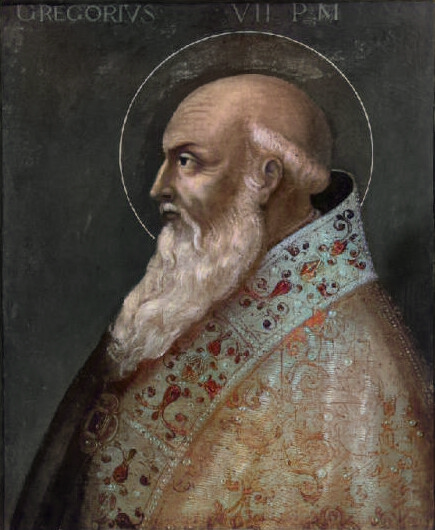
\includegraphics[width=\linewidth]{rehor_vii.png}
    \captionof{figure}{Řehoř VII.}
\end{minipage}


\subsection*{Štaufská dynastie (1138 -- 1250)}
\begin{minipage}{0.6\textwidth}
    \begin{itemize}
        \vspace{-0.5em}
        \setlength\itemsep{0.15em}
        \item[$-$] \textbf{Fridrich I. Barbarossa}
            \begin{itemize}
                \vspace{-0.5em}
                \setlength\itemsep{0.15em}
                \item[$-$] další snaha o oslabení církve, neúspěšné
                \item[$-$] chtěl se zmocnit S Itálie: 5 výprav
                \item[1158] Milán, pomáhá \textbf{Vladislav II.} -- opět jmenován králem
                \item[1176] \textsc{bitva u Leguna} výhra spojených severoitalských měst a papeže
                \item[$-$] Jindřich Lev z rodu Welfů, soupeří s J. B., poražen, musí odejít, jeho majetek rozdělen šlechtě
                \item[$-$] syn \textbf{Jindřich VI.} (žena Konstancie, dědička Sicílie)
                \item[$-$] zřídil Moravské markrabství, podléhá jemu $\rightarrow$ vymaní Moravu z vlivu českých knížat
                \item[$-$] pražského biskupa povýšil na říšského biskupa $\rightarrow$ nepodléhá českému králi
                \item[$-$] účast na \textit{třetí křížové výpravě}, kde se utopil
            \end{itemize}
        \item[$-$] \textbf{Fridrich II.} (1197 -- 1250)
            \begin{itemize}
                \vspace{-0.5em}
                \setlength\itemsep{0.15em}
                \item[$-$] syn Jindřicha VI.
                \item[1212] \textsc{Zlatá bula sicilská}, Morava připojena k českým zemím
                \item[1214] \textsc{bitva u Bouvines}, poražení Welfů
                \item[$-$] království vzkvétá, akceptuje muslimy, univerzita v Neapoli (přírodní vědy), spory s papežem
                \item[$-$] po jeho smrti období bezvládí -- \textit{interregnum}
            \end{itemize}
        \item[1257] sbor 7 kurfiřtů (4 světští, 3 církevní) volí krále
        \begin{description}
            \vspace{-0.5em}
            \setlength\itemsep{0.15em}
            \item[světští:] vévoda saský, markrabě braniborský, falckrabě rýnský, český král
            \item[církevní:] arcibiskupové kolínský, trevírský, mohučský
        \end{description}
        \item[1273] tímto způsobem zvolen jako první \textbf{Rudolf Habsburský}
    \end{itemize}
\end{minipage}
\hfill
\noindent\begin{minipage}{0.3\textwidth}
    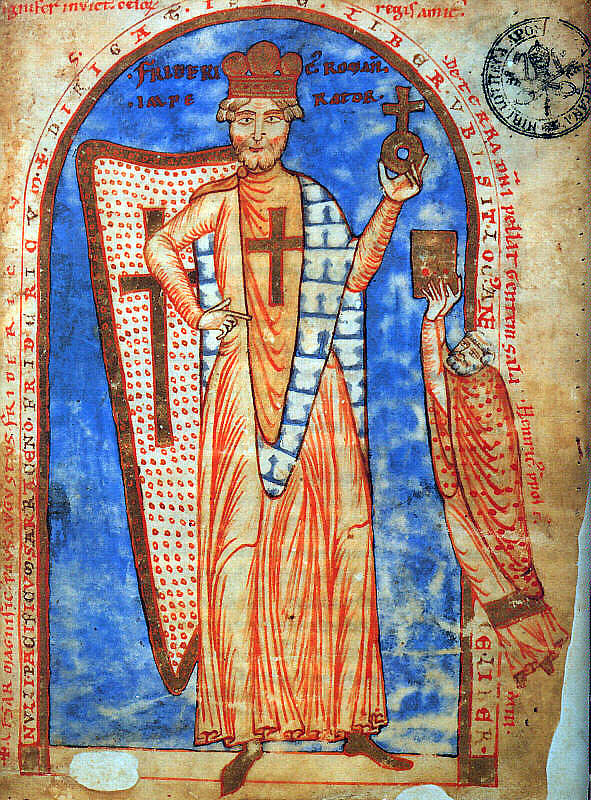
\includegraphics[width=\linewidth]{barbarossa.jpg}
    \captionof{figure}{Fridrich I. Barbarossa}
    \vspace{1em}
    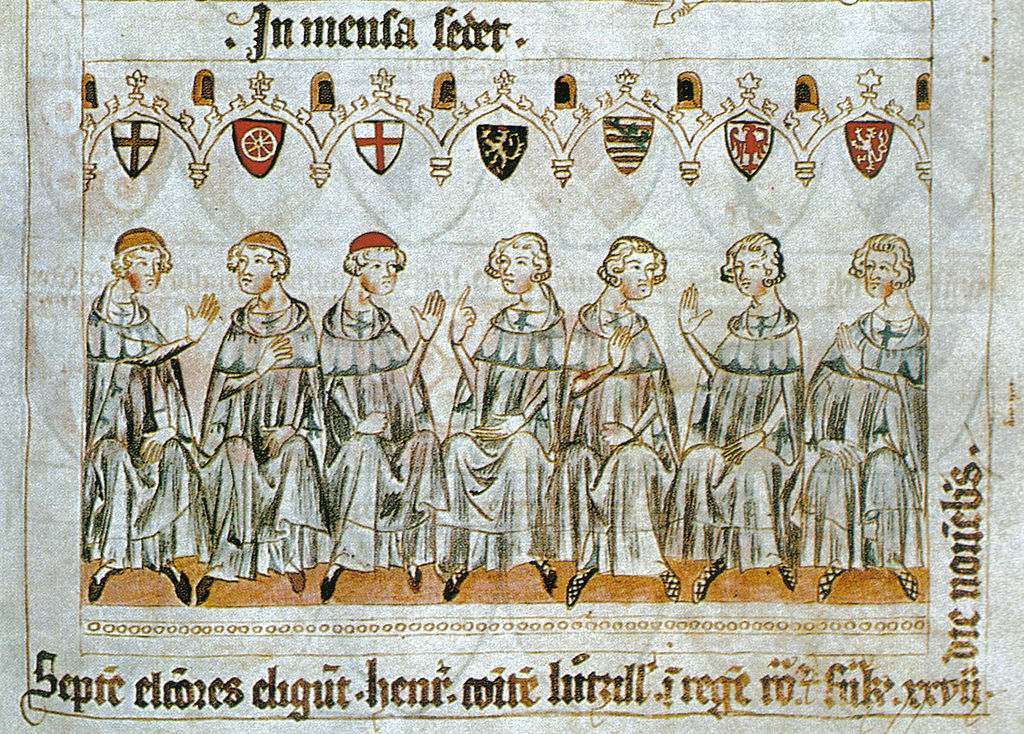
\includegraphics[width=\linewidth]{kurfirti.jpg}
    \captionof{figure}{Sbor volících kurfiřtů}
\end{minipage}
\end{document}
